\documentclass[czech, oth, kiv, he, iso690numb, viewonly]{fasthesis}
\usepackage[all]{hypcap} % \ref přesměruje uživatele na obrázek místo captionu obrázku
\usepackage{minted}
\usepackage{caption}
\usepackage{algorithm}
\usepackage{algpseudocode}
\usepackage{sourcecodepro}
\usepackage{amsmath}
\usepackage{dirtree}

\definecolor{codebg}{RGB}{240, 240, 240}

% Format the list of listings to have dots
\renewcommand{\listoflistings}{%
  \listof{listing}{Seznam výpisů}
  \addcontentsline{toc}{chapter}{Seznam výpisů}
  \label{lst:list_of_listings}
}

 % Set the label format for listings
\DeclareCaptionLabelFormat{mylisting}{Zdrojový kód #2}
\captionsetup[listing]{labelformat=mylisting}

\worktypespec{Semestrální práce}
\title{Překladač jazyka Ligma}
\author{Milan Janoch – janochmi@students.zcu.cz}{\\Jakub Pavlíček – jpvlck@students.zcu.cz}{Bc.}{}
\addbibresource{literatura.bib}

\begin{document}
\frontpages[tm]
\tableofcontents

    \chapter{Zadání}

    Cílem práce bude vytvoření překladače zvoleného jazyka. Je možné inspirovat se jazykem PL/0, vybrat si podmnožinu nějakého existujícího jazyka nebo si navrhnout jazyk zcela vlastní. Dále je také potřeba zvolit si pro jakou architekturu bude jazyk překládán (doporučeny jsou instrukce PL/0, ale je možné zvolit jakoukoliv instrukční sadu pro kterou budete mít interpret).
    \\\\
    Jazyk musí mít minimálně následující konstrukce:
    \begin{itemize}
        \item definice celočíselných proměnných
        \item definice celočíselných konstant
        \item přiřazení
        \item základní aritmetiku a logiku (+, -, *, /, \&\&, ||, !, (), ==, !=, <, >, <=, >=)
        \item cyklus (libovolný)
        \item jednoduchou podmínku (if bez else)
        \item definice podprogramu (procedura, funkce, metoda) a jeho volání
    \end{itemize}
    Překladač který bude umět tyto základní věci bude hodnocen deseti body. Další body (alespoň do minimálních 20) je možné získat na základě rozšíření, jsou rozděleny do dvou skupin, jednodušší za jeden bod a složitější za dva až tři body. Další rozšíření je možno doplnit po konzultaci, s ohodnocením podle odhadnuté náročnosti.
    \\\\
    Jednoduchá rozšíření (1 bod):
    \begin{itemize}
        \item každý další typ cyklu (for, do .. while, while .. do, repeat .. until, foreach)
        \item else větev
        \item datový typ boolean a logické operace s ním
        \item datový typ real (s celočíselnými instrukcemi)
        \item datový typ string (s operátory pro spojování řetězců)
        \item rozvětvená podmínka (switch, case)
        \item násobné přiřazení: a = b = c = d = 3;
        \item ternární operátor: min = (a < b) ? a : b;
        \item paralelní přiřazení \{a, b, c, d\} = \{1, 2, 3, 4\};
        \item příkazy pro vstup a výstup (read a write)
    \end{itemize}
    Složitěší rozšíření (2 body):
    \begin{itemize}
        \item příkaz GOTO (pozor na vzdálené skoky)
        \item datový typ ratio (s celočíselnými instrukcemi)
        \item složený datový typ (Record)
        \item pole a práce s jeho prvky
        \item operátor pro porovnání řetězců
        \item parametry předávané hodnotou
        \item návratová hodnota podprogramu
        \item objekty bez polymorfismu
        \item anonymní vnitřní funkce (lambda výrazy)
    \end{itemize}
    Rozšíření vyžadující složitější instrukční sadu než má PL/0 (3 body):
    \begin{itemize}
        \item dynamicky přiřazovaná paměť - práce s ukazateli
        \item parametry předávané odkazem
        \item objektové konstrukce s polymorfním chováním
        \item instanceof operátor
        \item anonymní vnitřní funkce (lambda výrazy) které lze předat jako parametr
        \item mechanismus zpracování výjimek
    \end{itemize}
    Vlastní interpret (řádkový, složitý alespoň jako rozšířená PL/0) je za 6 bodů. 
    \\\\
    Zohledňují se i další věci, které mohou pozitivně nebo negativně ovlivnit bodování:
    \begin{itemize}
        \item testování: tvorba rozumné automatické testovací sady +3 body
        \item kvalita dokumentace: -x bodů až +2 body podle kvality a prohřešků
        \item využití GITu: -x bodů až +2 body podle důslednosti a struktury příspěvků
        \item kvalita zdrojového textu: -x bodů až +2 body podle obecně známých pravidel
    \end{itemize}

    \chapter{Návrh jazyka}

    \section{Zvolená rozšíření jazyka Ligma}
    \begin{itemize}
        \item cyklus for
        \item cyklus do-while
        \item cyklus repeat-until
        \item datový typ boolean a logické operace s ním
        \item else větev
        \item násobné přiřazení: a = b = c = d = 3;
        \item parametry předávané hodnotou
        \item návratová hodnota podprogramu
    \end{itemize}

    \section{Omezení jazyka}
    \begin{itemize}
        \item Při deklaraci proměnné je třeba vždy nastavit hodnotu
        \item V hlavičce for cyklu se musí deklarovat proměnná
        \item Podporované datové typy: int, boolean
        \item Identifikátor nesmí obsahovat speciální znaky (kromě '\_') a začínat číslem
        \item Funkce musí být definovány až pod samotnými příkazy
        \item Funkce lze definovat pouze v globálním rozsahu
        \item Funkce musí vždy vracet hodnotu (return je vždy poslední příkaz funkce)
    \end{itemize}

    \section{Konstrukce jazyka}

    \subsection{Povinné}

    \subsubsection*{Definice celočíselných proměnných}
    \begin{minted}[fontsize=\footnotesize, numbersep=6pt, bgcolor=codebg]{cpp}
int a = 5;
    \end{minted}

    \subsubsection*{Definice celočíselných konstant}
    \begin{minted}[fontsize=\footnotesize, numbersep=6pt, bgcolor=codebg]{cpp}
const int a = 5;
    \end{minted}

    \subsubsection*{Přiřazení}
    \begin{minted}[fontsize=\footnotesize, numbersep=6pt, bgcolor=codebg]{cpp}
int a = 1;
a = 5;
    \end{minted}

    \subsubsection*{Základní aritmetika a logika}
    Aritmetika:
    \begin{minted}[fontsize=\footnotesize, numbersep=6pt, bgcolor=codebg]{cpp}
int a = 5 + 1;
int b = 5 - 1;
int c = 5 / 1;
int d = 5 * 1;
int e = -1;
int f = +1;
int g = 5 % 5;
    \end{minted}
    Logika:
    \begin{minted}[fontsize=\footnotesize, numbersep=6pt, bgcolor=codebg]{java}
boolean a = 1 < 5;
boolean b = 1 <= 5;
boolean c = 1 >= 5;
boolean d = 1 > 5;
boolean e = 1 == 5;
boolean f = 1 != 5;
boolean g = true && true;
boolean h = true || false;
    \end{minted}

    \subsubsection*{While cyklus}
    \begin{minted}[fontsize=\footnotesize, numbersep=6pt, bgcolor=codebg]{cpp}
int a = 0;

while (a < 5) {
    a = a + 1;
}
    \end{minted}

    \subsubsection*{Podmínka if (bez else)}
    \begin{minted}[fontsize=\footnotesize, numbersep=6pt, bgcolor=codebg]{cpp}
if (true) {
    ...
}
    \end{minted}

    \subsubsection*{Definice funkce a její volání}
    \begin{minted}[fontsize=\footnotesize, numbersep=6pt, bgcolor=codebg, extrakeywords={func}]{java}
int res = foo();

func int foo() {
    return 5;
}
    \end{minted}

    \subsection{Rozšiřující}

    \subsubsection*{Cyklus do-while}
    \begin{minted}[fontsize=\footnotesize, numbersep=6pt, bgcolor=codebg]{cpp}
int a = 1;

do {
    a = a + 1;
} while (a < 5);
    \end{minted}

    \subsubsection*{Cyklus repeat-until}
    \begin{minted}[fontsize=\footnotesize, numbersep=6pt, bgcolor=codebg, extrakeywords={repeat, until}]{cpp}
int a = 1;

repeat {
    a = a + 1;
} until (a >= 5);
    \end{minted}

    \subsubsection*{Cyklus for}
    Automaticky inkrementuje definovanou proměnnou v hlavičce (zde \glqq\texttt{a}\grqq) o 1.
    Vždy se porovnává, zda proměnná \glqq\texttt{a}\grqq \,je menší než hodnota výrazu za tokenem \glqq\texttt{to}\grqq.
    \begin{minted}[fontsize=\footnotesize, numbersep=6pt, bgcolor=codebg]{cpp}
for (int a = 0 to 10) {
    ...
}
    \end{minted}

    \subsubsection*{Else větev}
    \begin{minted}[fontsize=\footnotesize, numbersep=6pt, bgcolor=codebg]{java}
if (false) {
    ...
} else {
    ...
}
    \end{minted}

    \subsubsection*{Datový typ boolean a logické operace s ním}
    \begin{minted}[fontsize=\footnotesize, numbersep=6pt, bgcolor=codebg]{java}
boolean a = true;
boolean b = false;
boolean c = a && b;
boolean d = a || b;
boolean e = !a;
boolean f = true == false;
boolean g = true != false;
    \end{minted}

    \subsubsection*{Násobné přiřazení}
    Nejdříve se vyhodnocuje výraz na pravé straně.
    \begin{minted}[fontsize=\footnotesize, numbersep=6pt, bgcolor=codebg]{java}
int a = 1;
int b = 2;

a = b = 5;
    \end{minted}

    \subsubsection*{Parametry předávané hodnotou}
    \begin{minted}[fontsize=\footnotesize, numbersep=6pt, bgcolor=codebg, extrakeywords={func}]{java}
int res = foo(3, 4);
    
func int foo(int a, int b) {
    return a * b;
}
    \end{minted}

    \subsubsection*{Návratová hodnota podprogramu}
    \begin{minted}[fontsize=\footnotesize, numbersep=6pt, bgcolor=codebg, extrakeywords={func}]{java} 
int res = foo(1);

func int foo(int a) {
    return a - 1;
}
    \end{minted}

    \subsection{Vlastní}

    \subsubsection*{Mocnina}
    \begin{minted}[fontsize=\footnotesize, numbersep=6pt, bgcolor=codebg]{java}
int a = 2 ^ 5;
    \end{minted}

    \subsubsection*{Komentáře}
    \begin{minted}[fontsize=\footnotesize, numbersep=6pt, bgcolor=codebg]{java}
// Line comment

/*
    Multiline comment
*/
    \end{minted}

    \chapter{Implementace}

    K vytvoření překladače jazyka Ligma jsme použili nástroj ANTLR a programovací jazyk Java.
    Zdrojové soubory se nachází v adresáři \texttt{/ligma/src/}.
    Při implementaci byl používán nástroj Git pro verzování kódu a správu změn.
    Odkaz na GitHub repozitář: \url{https://github.com/M1LNES/FJP-semester-work}.

    \section{Struktura projektu}

    \dirtree{%
        .1 src.
        .2 main.
        .3 java.
        .4 ligma.
        .5 enums\DTcomment{výčtové typy (PL/0 instrukce, datové typy, ...)}.
        .5 exception\DTcomment{vlastní definované výjimky}.
        .5 generated\DTcomment{soubory vygenerované ANTLR za překladu}.
        .5 generator\DTcomment{generátory PL/0 instrukcí}.
        .5 ir\DTcomment{vnitřní reprezentace jazyka}.
        .5 listener\DTcomment{listenery pro lexikální/syntaktickou analýzu}.
        .5 table\DTcomment{tabulka symbolů}.
        .5 visitor\DTcomment{třídy pro průchod derivačního stromu}.
        .5 App.java\DTcomment{vstupní bod programu}.
        .3 resources.
        .4 output.\DTcomment{výstupy programů (PL/0 instrukce)}.
        .4 programs.\DTcomment{ukázkové programy}.
        .2 test.
        .3 java.\DTcomment{testy}.
        .3 resources.\DTcomment{testovací soubory}.
    }

    \pagebreak

    \section{Lexikální a syntaktická analýza}

    Gramatika jazyka, definovaná v souboru \texttt{Ligma.g4}, popisuje lexikální a syntaktická pravidla pro překladač.
    Obsahuje pravidla pro klíčová slova, datové typy, literály, operátory a struktury, jako jsou cykly, podmínky, funkce a přiřazení hodnot.
    Zmíněný soubor tvoří základ pro generování derivačního stromu, který je dále využíván v překladači.
    
    Lexikální část gramatiky (\texttt{lexer rules}) rozpoznává jednotlivé tokeny, zatímco syntaktická část (\texttt{parser rules}) určuje hierarchii a strukturu příkazů. 
    Gramatika je navržena tak, aby umožnila parsování komplexních výrazů včetně operátorů s~různou prioritou. 

    Pro kontrolu chyb během lexikální a syntaktické analýzy jsme vytvořili vlastní listenery v balíčku \texttt{listener}.
    Ty zachycují chyby a vytváří výjimky, které obsahují informace o chybě v kódu.

    \section{Sémantická analýza}

    Sémantická analýza je prováděna v průběhu průchodu derivačního stromu.
    V rámci sémantické analýzy jsou kontrolována pravidla jazyka, jako je např. kontrola deklarace proměnných, kontrola typů operandů, atd.
    V případě nalezení chyby je vyhozena výjimka, která obsahuje informace o chybě v kódu.
    Během sémantické analýzy je vytvářena vnitřní reprezentace jazyka, která je následně použita pro generování PL/0 instrukcí.

    Pro sémantickou analýzu slouží třídy v balíčku \texttt{visitor}.
    Tyto třídy implementují rozhraní \texttt{LigmaBaseVisitor}, které obsahuje metody pro každý typ uzlu v derivačním stromu.
    Uvnitř těchto metod je prováděna sémantická analýza.

    \subsection{Tabulka symbolů}

    Během sémantické analýzy se také vytváří tabulka symbolů, která obsahuje informace o deklarovaných proměnných a funkcích.
    Tabulka symbolů je implementována jako zásobník rozsahů, kde každý blok (např. funkce, cyklus) má svůj vlastní rozsah (scope).
    Každý rozsah pak obsahuje mapu identifikátorů a jejich příslušných informací (datový typ, adresa, ...).
    Díky tomu je možné jednoduše získat informace o proměnných a funkcích v rámci daného bloku.

    \pagebreak

    \section{Generování PL/0 instrukcí}

    Generování PL/0 instrukcí je prováděno pomocí vnitřní reprezentace jazyka, která byla dříve vytvářena sémantickou analýzou.
    Vnitřní reprezentace obsahuje informace o jednotlivých částech programu, které jsou následně převedeny do instrukcí jazyka PL/0.
    Generování instrukcí je prováděno v balíčku \texttt{generator}, přičemž výsledné instrukce jsou ukládány do souboru.

    \subsection{Generování funkcí}

    Jednotlivé funkce jsou generovány jen v případě, že je daná funkce volána.
    Instrukce funkce se tak po jejím zavolání nachází \glqq uvnitř\grqq \,samotného volání, což lze chápat jako rozvinutí makra v daném místě.
    Přičemž pomocí pomocné mapy funkcí je zařízeno, že během generování volání funkce se nastaví správná adresa začátku funkce.
    Pokud je ale stejná funkce volána vícekrát, je generována pouze jednou.

    \subsection{Generování mocniny}

    Generování mocniny jsme vyřešili pomocí \glqq pomocné\grqq \,funkce, která v sobě obsahuje cyklus, který násobí hodnotu základu tolikrát, kolik je hodnota exponentu.
    Díky tomu byla zajištěna izolace pomocných proměnných a zároveň bylo dosaženo správného výsledku.
    Ve výrazu mocniny se tak můžou nacházet jak hodnoty, proměnné, tak různě složité výrazy.

    \pagebreak

    \subsection{Výsledná implementace}

    Výslednou implementaci lze popsat následujícím pseudokódem:

    \begin{algorithm}
        \caption{Překladač jazyka Ligma}\label{alg:cap}
        \begin{algorithmic}
            \State \textbf{Fáze 1: Lexikální analýza}
            \State \textbf{Vstup:} Zdrojový kód v jazyce Ligma
            \State \textbf{Výstup:} Seznam tokenů
            \For{každý znak v kódu}
                \State \textbf{Pokud} neplatný znak, \textbf{pak} generuj chybu, \textbf{jinak} vytvoř token
            \EndFor
            \\
            \State \textbf{Fáze 2: Syntaktická analýza}
            \State \textbf{Vstup:} Seznam tokenů
            \State \textbf{Výstup:} Derivační strom
            \For{každý token}
                \State \textbf{Pokud} token neodpovídá syntaxi, \textbf{pak} generuj chybu, \textbf{jinak} vytvoř uzel
            \EndFor
            \\
            \State \textbf{Fáze 3: Sémantická analýza}
            \State \textbf{Vstup:} Derivační strom
            \State \textbf{Výstup:} Vnitřní reprezentace jazyka a kontrola sémantiky/typů
            \For{každý uzel ve stromě}
                \State \textbf{Pokud} chyba sémantiky/typu, \textbf{pak} generuj chybu, \textbf{jinak} vytvoř vnitřní reprezentaci
            \EndFor
            \\
            \State \textbf{Fáze 4: Generování PL/0 instrukcí}
            \State \textbf{Vstup:} Vnitřní reprezentace jazyka
            \State \textbf{Výstup:} Soubor s PL/0 instrukcemi
            \For{každý objekt}
                \State \textbf{Pokud} chyba při generování, \textbf{pak} generuj chybu, \textbf{jinak} vygeneruj instrukce
            \EndFor
        \end{algorithmic}
    \end{algorithm}

    \chapter{Testování}

    Projekt obsahuje sadu automatických testů, které testují lexikální, syntaktickou a~sémantickou analýzu.
    Všechny testy (celkem \textbf{242}) jsou automaticky spouštěné při vytváření výsledného \texttt{.jar} souboru pomocí skriptu \texttt{run.sh} (případně \texttt{run.bat} na Windows).
    Testování bylo prováděno na operačních systémech Windows a macOS.
    Testy se nachází v adresáři \texttt{/src/test} (dále uvažujme tento soubor).

    Kód překladač zahrnuje logování důležitých informací o průběhu sémantické analýzy a generování instrukcí.
    Díky důkladnému logování jsme bylo schopni snadno identifikovat chyby a problémy v kódu.

    \section{Lexikální analýza}

    Testy pro lexikální analýzu spouští třída \texttt{ExpressionLexicalTest}.
    Obsahuje celkem \textbf{12} negativních testů, které validují správnou funkčnost lexikální analýzy.
    Testovací soubory se nachází v adresáři \texttt{resources/lexical}.

    \section{Syntaktická analýza}

    Testy pro syntaktickou analýzu spouští třída \texttt{ExpressionSyntaxTest}.
    Obsahuje celkem \textbf{148} testů (pozitivních + negativních).
    Testovací soubory se nachází v adresáři \texttt{resources/syntax}.
    Důraz u negativních testů byl kladen zejména na provádění neplatných operací (např. chybějící operandy/operátory) či používání neplatných instrukcí.

    \section{Sémantická analýza}

    Testy pro sémantickou analýzu spouští třídy \texttt{ExpressionSemanticTest} a \texttt{FunctionSemanticTest}.
    Tyto třídy testují sémantiku a zároveň kontrolují typové chyby výrazů a funkcí.
    Obsahují celkem \textbf{72} testů (pozitivních + negativních).
    Testovací soubory se nachází v adresáři \texttt{resources/semantic}.

    \section{Generování PL/0 instrukcí}

    Testy pro generování PL/0 instrukcí spouští třída \texttt{ExpressionGeneratorTest}.
    Tato třída vezme ukázkové soubory (celkem \textbf{10}) uvedené v adresáři \texttt{/programs} a vygeneruje z nich PL/0 instrukce do stejnojmenných souborů v adresáři \texttt{/output}.
    Tímto je zaručeno, že při spuštění skriptu \texttt{run.sh} (případně \texttt{run.bat} na Windows) budou opětovně vygenerovány PL/0 instrukce pro všechny ukázkové programy.
    Zároveň je zaručeno, že nedojde k žádné chybě při generování instrukcí z ukázkových souborů.
    
    Ukázkové zdrojové kódy přeložené do instrukční sady PL/0 se nachází v adresáři \texttt{/src/main/resources} –
    adresář \texttt{/programs} obsahuje zdrojové kódy jazyka Ligma a adresář \texttt{/output} vygenerované \texttt{PL/0} instrukce.

    \section{Zhodnocení}

    Výsledná implementace byla otestována celkem \textbf{242} testy, které pokrývají všechny části jazyka Ligma.
    Díky rozsáhlé sadě testů bylo možné identifikovat a odstranit chyby v kódu.
    Výsledky testování jsou zobrazeny v tabulce a grafu na obr. \ref{fig:tests}.

    \begin{figure}[ht]
        \centering
        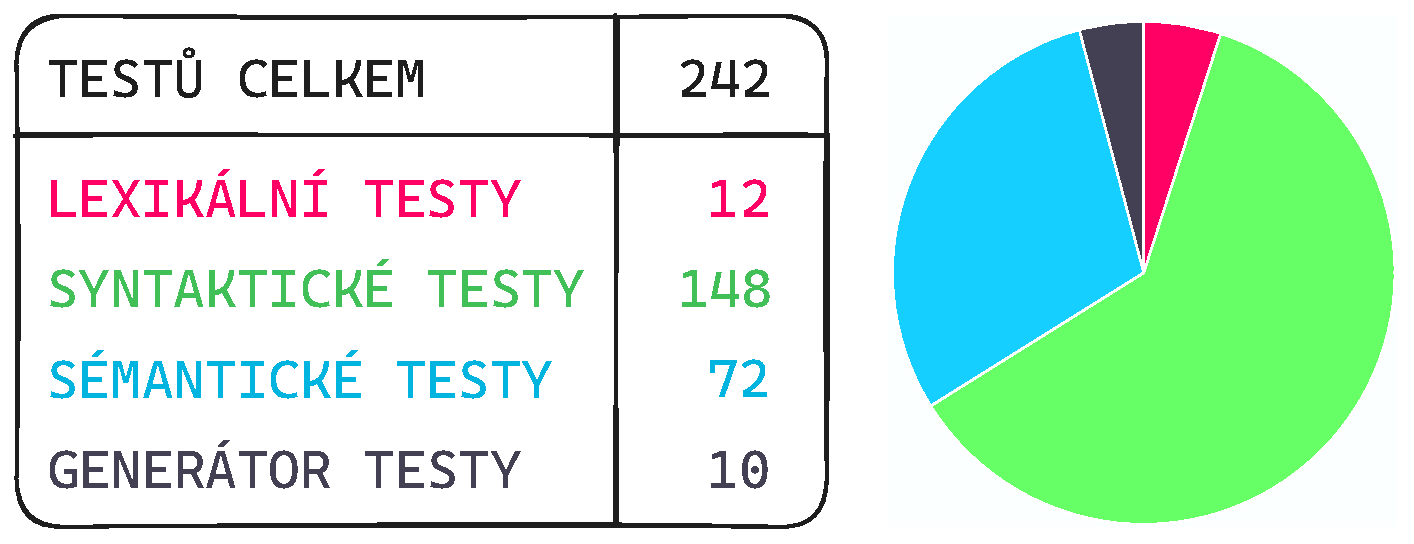
\includegraphics[width=0.8\textwidth]{images/testy.pdf}
        \caption{Výsledný počet testů}
        \label{fig:tests}
    \end{figure}

    \chapter{Uživatelská dokumentace}

    \section{Prerekvizity}

    Pro úspěšné přeložení je vyžadováno:
    \begin{itemize}
        \item Java verze 23 (kvůli podpoře Markdown komentářů)
        \item Maven verze 3.9.9
    \end{itemize}

    \section{Instalace a spouštění}

    \begin{enumerate}
        \item \textbf{Otevření adresáře s aplikací}
            \begin{itemize}
                \item Otevřete adresář \texttt{ligma}: \mintinline[fontsize=\footnotesize, numbersep=6pt, bgcolor=codebg]{bash}|cd ligma|
            \end{itemize}
        \item \textbf{Instalace a spuštění}
            \begin{itemize}
                \item Pro \textbf{Windows}: \mintinline[fontsize=\footnotesize, numbersep=6pt, bgcolor=codebg]{bash}|run.bat|
                \item Pro \textbf{Linux} a \textbf{macOS}: \mintinline[fontsize=\footnotesize, numbersep=6pt, bgcolor=codebg]{bash}|sh run.sh|
            \end{itemize}
    \end{enumerate}
    Skript spustí příkaz \texttt{mvn clean install}, který stáhne veškeré potřebné knihovny, přeloží projekt (vytvoří adresář \texttt{/target} s přeloženými soubory), následně spustí testy a vytvoří finální spustitelný soubor \texttt{ligma.jar} jak v aktuálním adresáři, tak v~adresáři \texttt{/target}. 
    
    Nakonec se spustí ukázkový program a vygeneruje se výstupní soubor s PL/0 instrukcemi.
    Ve skriptu je možné upravit cestu k ukázkovému programu, který se má přeložit. Díky spuštěným testům je však zaručeno, že se opětovně vygenerují PL/0 instrukce pro všechny ukázkové programy.
    \\\\
    Program lze spustit i bez použití skriptu, a to příkazem:
    \begin{minted}[fontsize=\footnotesize, numbersep=6pt, bgcolor=codebg]{bash}
java -jar ligma.jar <input-file> <output-file>
    \end{minted}
    kde \texttt{<input-file>} je cesta k souboru se zdrojovým kódem jazyka Ligma a \texttt{<output-file>} je výsledný soubor s \texttt{PL/0} instrukcemi.

    \chapter{Závěr}

    V rámci semestrální práce byl úspěšně vytvořen funkční překladač jazyka Ligma do instrukcí PL/0.
    
    Navrhli jsme si vlastní jazyk Ligma, který je popsán gramatikou \texttt{Ligma.g4}.
    Z~gramatiky je pak nástrojem ANTLR vygenerován derivační strom, který je možné dále procházet či zpracovávat.
    Při průchodu derivačního stromu jsou kontrolována pravidla jazyka a zároveň je vytvářena vnitřní reprezentace jazyka v podobě objektů.
    Z~vnitřní reprezentace jsou následně generovány instrukce jazyka PL/0.
    Celý průběh překladu je podrobně logován do konzole.
    
    Pro testování vygenerovaných instrukcí ukázkových programů byl využit on-line interpret \url{https://home.zcu.cz/~lipka/fjp/pl0/}.
    Výsledný překladač byl otestován velkou sadou testů, které pokrývají všechny části jazyka Ligma.

    \appendix

    \printbibliography
        
    \backmatter
    \listoffigures

\end{document}